\documentclass[12pt, a4paper]{report}


\usepackage[T1]{fontenc}
\usepackage[latin1]{inputenc}
\usepackage[english]{babel}
\usepackage{siunitx}
\usepackage{graphicx}
\usepackage{tipa} % for the \ark{} command
\usepackage{graphics} % for pdf, bitmapped graphics files
\usepackage{times} % assumes new font selection scheme installed
\usepackage{amsmath}
\usepackage{latexsym}
\usepackage{amscd}% for commutative diagrams
\usepackage{mathrsfs} %this package is for the script font \mathscr
\usepackage{relsize}
\usepackage{delarray}
\usepackage{pstricks}
\usepackage{theorem}
\usepackage{changepage}
\usepackage{euscript}
\usepackage{textcomp}
\usepackage{esvect}
\usepackage{parskip}
\usepackage{placeins}
\usepackage{subfigure}
% \usepackage{subcaption}
\usepackage{array}
\usepackage{delarray}
\usepackage{stmaryrd}
\usepackage{fancyhdr}
\usepackage{graphpap}
\usepackage{makeidx}
\usepackage{enumerate}
\usepackage{esint}
\usepackage{datetime}
\usepackage{caption}
\usepackage{smartdiagram}
\usesmartdiagramlibrary{additions}
%Set Abstract Page
\usepackage{abstract}
\setlength{\absleftindent}{-5mm}
\setlength{\absrightindent}{-5mm}

%Colour definitions - put before TikZ
\usepackage{color}
\definecolor{igreen}{rgb}{0.0, 0.56, 0.0}
\usepackage{xcolor, colortbl}
\colorlet{gred}{-red!75!green!65!}
\colorlet{mamber}{-red!75!green!15!blue!50!}
\colorlet{grown}{-red!75!blue!20!green}
\colorlet{bled}{-red!85!blue!40!green!45!}
\colorlet{waters}{cyan!25} % Define color for the water
\colorlet{water}{cyan!25!green!20!} % Define color for the water
\definecolor{grin}{HTML}{00F9DE}
\usepackage{rotating}
\providecommand{\keywords}[1]{\textbf{\textit{Keywords---}} #1}

% For faint dotted table line
\usepackage{arydshln}
\setlength{\dashlinedash}{.4pt}
\setlength{\dashlinegap}{.8pt}

\usepackage{booktabs}
\usepackage{graphicx}
\usepackage{tikz}
\usepackage{tikz-3dplot}
\usetikzlibrary{
arrows,
arrows.meta,
automata,
backgrounds,
calc,
decorations,
decorations.pathmorphing,
decorations.pathreplacing,
decorations.fractals,
external,
fit,
matrix,
petri,
positioning,
shadows,
shapes,
shapes.multipart,
topaths,
intersections
}
\usepackage{eso-pic}
\def\ba{\begin{array}}
\def\ea{\end{array}}
\def\beann{\begin{eqnarray*}}
\def\eeann{\end{eqnarray*}}
\def\bea{\begin{eqnarray}}
\def\eea{\end{eqnarray}}
\def\bsy{\boldsymbol}
\def\gray#1{{\color{gray}#1}}

%% COUNTERS
\setcounter{MaxMatrixCols}{20}
\renewcommand{\thesection}{\arabic{section}}
\renewcommand{\thesection}{\thechapter.\number\numexpr\value{section}}
\renewcommand{\thesubsection}{\thesection.\number\numexpr\value{subsection}}
%%For changemargin
\def\quote{\list{}{\rightmargin\leftmargin}\item[]}
\let\endquote=\endlist 
\def\changemargin#1#2{\list{}{\rightmargin#2\leftmargin#1}\item[]}
\let\endchangemargin=\endlist 
\makeatletter
\newlength\qvec@height
\newlength\qvec@depth
\newlength\qvec@width
\newcommand{\qvec}[2][]{
    \settoheight{\qvec@height}{$#2$}
    \settodepth{\qvec@depth}{$#2$}
    \settowidth{\qvec@width}{$#2$}
  \def\qvec@arg{#1}
  \raisebox{.2ex}{\raisebox{\qvec@height}{\rlap{% 
    \kern.05em
    \begin{tikzpicture}[scale=1,shorten >=-3pt,shorten <=-3pt]
    \pgfsetroundcap
    \coordinate (Stx) at (.05em,0) ;
		\coordinate (Arx) at (\qvec@width-.05em,0) ;
    \draw[->](Stx) to[bend left] (Arx);
    \end{tikzpicture}
  }}}
  #2
}
\makeatother
\makeatletter
\newlength\pvec@height
\newlength\pvec@depth
\newlength\pvec@width
\newcommand{\pvec}[2][]{
    \settoheight{\pvec@height}{$#2$}
    \settodepth{\pvec@depth}{$#2$}
    \settowidth{\pvec@width}{$#2$}
  \def\pvec@arg{#1}
  \raisebox{.2ex}{\raisebox{\pvec@height}{\rlap{% 
    \kern.05em
    \begin{tikzpicture}[scale=1,shorten >=-3pt,shorten <=-3pt]
    \pgfsetroundcap
    \coordinate (Stx) at (.05em,0) ;
		\coordinate (Arx) at (\pvec@width-.05em,0) ;
    \draw[->](Stx) to[bend right] (Arx);
    \end{tikzpicture}
  }}}
  #2
}
\makeatother
\makeatletter
\newlength\vvec@height%
\newlength\vvec@depth%
\newlength\vvec@width%
\newcommand{\vvec}[2][]{%
  \ifmmode%
    \settoheight{\vvec@height}{$#2$}%
    \settodepth{\vvec@depth}{$#2$}%
    \settowidth{\vvec@width}{$#2$}%
  \else 
    \settoheight{\vvec@height}{#2}%
    \settodepth{\vvec@depth}{#2}%
    \settowidth{\vvec@width}{#2}%
  \fi%
  \def\vvec@arg{#1}%
  \def\vvec@dd{:}%
  \def\vvec@d{.}%
  \raisebox{.2ex}{\raisebox{\vvec@height}{\rlap{%
    \kern.05em%
    \begin{tikzpicture}[scale=1]
    \pgfsetroundcap
    \draw (.05em,0)--(\vvec@width-.05em,0);
    \draw (\vvec@width-.05em,0)--(\vvec@width-.15em, .075em);
    \draw (\vvec@width-.05em,0)--(\vvec@width-.15em,-.075em);
    \ifx\vvec@arg\vvec@d%
      \fill(\vvec@width*.45,.5ex) circle (.5pt);%
    \else\ifx\vvec@arg\vvec@dd%
      \fill(\vvec@width*.30,.5ex) circle (.5pt);%
      \fill(\vvec@width*.65,.5ex) circle (.5pt);%
    \fi\fi%
    \end{tikzpicture}%
  }}}%
  #2%
}
\makeatother
\def\ba{\begin{array}}
\def\ea{\end{array}}
\def\beann{\begin{eqnarray*}}
\def\eeann{\end{eqnarray*}}
\def\bea{\begin{eqnarray}}
\def\eea{\end{eqnarray}}
\def\bsy{\boldsymbol}
\def\gray#1{{\color{gray}#1}}
\usepackage{titlesec}
\usepackage{multirow}
%To reference within text
\usepackage{hyperref}
\usepackage{apacite}
\usepackage{lipsum}
\usepackage{tikz-cd}
\usepackage{float}
\usepackage{titling}
\usepackage{epigraph}
\usepackage[title, titletoc]{appendix}
\setlength\epigraphwidth{8cm}
\setlength\epigraphrule{0pt}

\titleformat{\chapter}{\normalfont\LARGE}{\thechapter\,$\vert$}{20pt}{\LARGE}{\setcounter{chapter}{0}}
\setlength{\headheight}{15pt}
\titlespacing*{\chapter}{0pt}{-70pt}{40pt} %Move chapter titles up
% Title page logos:
\makeatletter
\newcommand\BackgroundPicturea[3]{
	\setlength{\unitlength}{1pt}
	\put(0,\strip@pt\paperheight){
		\parbox[t]{\paperwidth}{
			\vspace{#2}\hspace{#3}
			\mbox{\includegraphics[scale=0.5]{#1}}
}}}
\newcommand\BackgroundPictureb[3]{
	\setlength{\unitlength}{1pt}
	\put(0,\strip@pt\paperheight){
		\parbox[t]{\paperwidth}{
			\vspace{#2}\hspace{#3}
			\mbox{\includegraphics[scale=0.3]{#1}}
}}}
\makeatother
% For my abbreviations
\newcommand{\abbrlabel}[1]{\makebox[3cm][l]{\textbf{#1}\ \dotfill}}
\newenvironment{abbreviations}{\begin{list}{}{\renewcommand{\makelabel}{\abbrlabel}}}{\end{list}}
% Line Spacing
\usepackage{setspace}
\setstretch{1.5}
%Set of command is for the changemargin environment
\def\quote{\list{}{\rightmargin\leftmargin}\item[]}
\let\endquote=\endlist 
\def\changemargin#1#2{\list{}{\rightmargin#2\leftmargin#1}\item[]}
\let\endchangemargin=\endlist
%Replace Contents to Table of Contents	
\addto\captionsenglish{
	\renewcommand{\contentsname}%
	{Table of Contents}
	\setcounter{tocdepth}{3}% Include \subsubsection in ToC
	\setcounter{secnumdepth}{3}% Number \subsubsection in ToC
	}
\renewcommand{\listfigurename}{List of Figures}
\renewcommand{\listtablename}{List of Tables}


\theoremstyle{definition}
\newtheorem{theorem}{Theorem}[section]

\theoremstyle{definition}
\newtheorem{definition}{Definition}[section]

\theoremstyle{definition}
\newtheorem{nproof}{Proof}[section]


\hypersetup{pdftitle = Project Report, pdfauthor = {First Last}, pdfstartview=FitH, pdfkeywords = essay, pdfpagemode=FullScreen, colorlinks, anchorcolor = red, citecolor = purple, urlcolor=blue, filecolor=green, linkcolor=blue, plainpages=false}
%%%%%%%%%%%%%%%%%%%%%%%%%%%%%%%%%%%%%%%%%%%%%%%%%%%%%%%%%%%%%%%%%%%%%%%
\pagestyle{fancy}
\rhead{Computer Science}
\chead{}
\lhead{University of Oxford}
\lfoot{\date{}}
\cfoot{}
\rfoot{\thepage}
% Top and Bottom Line Rules
\renewcommand{\headrulewidth}{0.4pt} %0.4pt
\renewcommand{\footrulewidth}{0.4pt}
\fancyheadoffset{9pt}
\fancyfootoffset{9pt}
% Line spacing
\renewcommand{\baselinestretch}{1.5} %1.5
%%%%%%%%%%%%%%%%%%%%%%%%%%%%%%%%%%%%%%%%%%%%%%%%%%%%%%%%%%%%%%%%%%%%%%%
\date{}

\title{Batch Active Learning using Deep Kernel Gaussian Process Classifiers}
\author{\\ \Large{Candidate Number: 1032626}
\\ Computer Science
\\
\\
\\
\\ University of Oxford
\\
\\ \\
Trinity 2021
}
%%%%%%%%%%%%%%%%%%%%%%%%%%%%%%%%%%%%%%%%%%%%%%%%%%%%%%%%%%%%%%%%%%%%%%%

\DeclareMathOperator{\E}{\mathbb{E}}

\begin{document}
% Adjust logo positions here
\AddToShipoutPicture*{\BackgroundPicturea{Logos/logo2.png}{0.7in}{5.8in}}

\thispagestyle{headings}
	\maketitle
\FloatBarrier
\pagenumbering{roman}


\thispagestyle{empty}
\begin{abstract}

This project report details extensions of various Batch Active Learning methods to the context of Deep Kernel - Multiclass Gaussian Processes Classification. By doing this we achieve SOTA active learning performance on MNIST.

We are also able to improve the computational cost of of each acquisition from being $O(n^3)$, related to the pool size if implemented directly to $O(n)$.


\keywords{Active Learning - Gaussian Processes - Deep Kernel Learning}
% \vspace{-10mm} %To remove added white space after
\end{abstract}
\tableofcontents
\thispagestyle{plain}
\listoffigures
\listoftables
\listofalgocfs
\listoftheorems
\chapter*{List of Abbreviations}
\begin{abbreviations}
    \item[GP] Gaussian Process
    \item[GPC] Gaussian Process Classification
    \item[BALD] Bayesian Active Learning by Disagreement
    \item[ELBO] Evidence Lower Bound
    \item[ML] Machine Learning
    \item[MNIST] Modified National Institute of Standards and Technology (A standard handwritten digit dataset)
    \item[BALD] Bayesian Active Learning by Disagreement
    \item[vDUQ] Variational Deterministic Uncertainty Quantification
    \item[DUE]   Deterministic Uncertainty Estimation
    \item[CUDA] Compute Unified Device Architecture
    \item[VRAM] Video Random Access Memory  
    \item[CIFAR10] A standard academic image classification dataset 
\end{abbreviations}

\chapter{Introduction}
\pagenumbering{arabic}

Active learning is an area of machine learning where we are attempting to select which unlabelled datapoints we believe would be best to learn the label of. It is important because in many important use cases (for example, medical data), it is often either quite costly or just simply impossible to collect an incredibly large dataset. However current approaches to do it suffer from issues related to quality of acquired datapoints, model requirements and computational issues.

Bayesian ML models are the standard ways of building machine learning models which can calculate uncertainty well, however many of the standard approaches to doing so (MC Dropout) can give suboptimal performance, for example requiring a substantial amount of sampling. Gaussian Processes are a ML approach which give very good uncertainty performance, and new results in the field [DUE] have shown successful training of Variational Gaussian Processes with feature extractors and demonstrate that they maintain good uncertainty performance.

\section{Motivation}

Active Learning is an active area of Machine Learning where we are trying to select (unlabelled) data points in an attempt to maximize some objective.
\section{Aim and Objectives}

The aims of this report is to

\begin{itemize}
    \item Give an outline of the various methods for Active Learning in the literature which we will be investigating
    \item Extend BathBald and related methods to Gaussian Process Classifiers with Deep Kernel Learning
    \item Reduce the computation required to perform these calculations to make it of practical use.
    \item Perform experiments to validate the performance of our created methods methods.
\end{itemize}
\section{Project Report Outline}
The remainder of this report is organized as follows:
\begin{itemize}
    \item[] \textbf{Chapter} \hyperref[sec:ActiveLearning]{\textbf{2}} --- Defines active learning, and introduces the different active learning methods from the literature.
    \item[] \textbf{Chapter} \hyperref[sec:Models]{\textbf{3}} --- Bayesian Machine Learning Models
    \item[] \textbf{Chapter} \hyperref[sec:DUE]{\textbf{4}} --- introduces Gaussian Process based models
    \item[] \textbf{Chapter} \hyperref[sec:ActiveLearningWithDUE]{\textbf{4}} --- introduces Gaussian Process based models 
    \item[] \textbf{Chapter} \hyperref[sec:Implementation]{\textbf{5}} --- Combines BatchBALD and GPC
    \item[] \textbf{Chapter} \hyperref[sec:Experiments]{\textbf{7}} --- Combines BatchBALD and GPC] 
\end{itemize}


\chapter{Active Learning Methods}
\label{sec:ActiveLearning}

In a common active learning formulation we have the following setup:

\begin{itemize}
    \item $X_{pool}$  is the distribution of the pool of points.
    \item $X_{true}$  is the true real world distribution.
\end{itemize}

A common (and sensible) assumption is to assume that these distributions are the same.

Our machine learning models, which we use to model a problem constrain the set of possible functions which we can represent and learn. This is how we imbue the problem with our prior beliefs about the nature of the problem.

\begin{itemize}
    \item There are hard constraints (eg. clipping the output of the model), which even given an unlimited amount of data our model can not possibly "learn around".
    \item There are softer constraints (eg. priors over weights in a layer), which our model can learn correctly given sufficient amounts of data even if our prior is poor*.
\end{itemize}

This parameterization of our models is very important, as this is an assumption we are making about our problem.

An important observation is that the dataset we are using for training is, unless we are performing very simple active learning approaches (eg. random acquisition) is not going to be the same as the true dataset which we are working with.

This violates a very common assumption that we assume for convergence in many ML methods. This statistical bias is looked at in the following paper \cite{farquhar2021statistical}.

When working with active learning, we are normally training our models on much smaller datasets than is standard in machine learning. Given our models are often over parameterized to begin with \cite{}, the smaller dataset will make this even more so, this can lead to training issues.

In the next sections we will describe the active learning methods which we will be investigating in this report.

\section{Random}

The most straightforward acquisition function is to randomly sample from the poolset. This is a surprisingly strong baseline for for many datasets. However random acquisition can have some failure modes in comparison to some other methods. 

An example of this failure can occur when only a small subset of the poolset contain useful new information. Datasets such as this can exist when the poolset is unbalanced, relative to the test set. The number of datapoints of a particular class which will be selected from the poolset will approximately in proportion.

\begin{figure}[H]
    \centering
    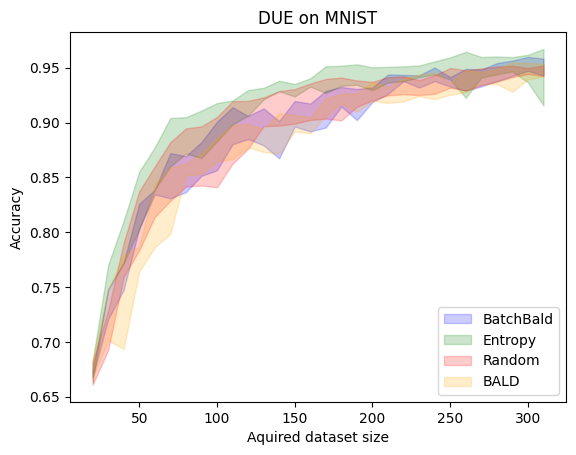
\includegraphics[scale=0.75]{random.png}
    \caption{Random MNIST vs Unbalanced MNIST}
\end{figure}

\section{BALD}
Bayesian Active Learning by Disagreement (BALD) \cite{houlsby2011bayesian} is an active learning method which is designed to select the datapoint which we expect would reduce the uncertainty of the posterior by the greatest amount if the value of $y$ at that point was known.


$${\argmax}_x H \left[ \theta | D \right] - \mathbf{E}_{y \sim p(y | x, D)} \left[ H\left[ \theta | y, x, D\right]\right]$$

To try and compute this directly we would have to attempt to calculate the entropy in the parameter space, however this is can be a very high dimensional space, however the authors of this paper observe that this objective can be rewritten as the conditional mutual information of the output variable and the parameters.

$$I \left(y, \theta| D, x \right) = H \left[ \theta | D \right] - \mathbf{E}_{y \sim p(y | x, D)} \left[ H\left[ \theta | y, x, D\right]\right]$$



By taking advantage of this formulation they then rewrite the objective as follows, which requires the computation of the entropy over the output variable instead which is normally over a much smaller dimensional space.


$${\argmax}_x H \left[ y | x, D \right] - \mathbf{E}_{\theta \sim p(\theta | D)} \left[ H\left[ y | x, \theta \right]\right]$$


An issue which we run into when using BALD in the case where we want to select multiple datapoints to acquire at the same time is the fact that selecting the $n$ points with the greatest individual information content will not necessarily give you the $n$ points which jointly have the greatest information content. This can be made very obvious by considering the case when there is duplicates in the dataset. If the duplicated point is in the top n points as decided by the BALD score, having both of the points in your acquired batch will give you no more information than just having one of them, you would be better served by selecting any other point instead of these points.

\section{BatchBALD}
BatchBALD \cite{kirsch2019batchbald}, is an extension of BALD designed especially to deal with the issues which we run into when using BALD to acquire batches of points.

To do this the objective function is modified, the original BALD objective is retained by setting $n = 1$ .

The BatchBALD score function is as follows.


\begin{definition}[BatchBALD]
    $$s_{BatchBald} (x_1, \ldots, x_n) = H(y_1, \ldots, y_n) - E_{p(f)}\left[H(y_1, \ldots, y_n | f)\right]$$
\end{definition}


\begin{definition}[Submodularity]
    A function $f : P(X) \rightarrow \mathbf{R}$ is sub modular if for all $A,B \subseteq X$ we have the following.

    $$f(A) + f(B) \geq f\left( A \cup B \right) +  f\left(A \cap B \right) $$
\end{definition}

The authors of the paper prove that the objective function that they specify is \textit{sub-modular}, which enables a greedy $1 - \frac{1}{\epsilon}$ approximation algorithm for selecting the optimum batch.



As the variables are independent conditioned on the value of the function, the right hand side of the equation factors into a sum over conditional expectations for each individual datapoint. The computationally difficult part of this objective is the computation of the joint entropy as this does not factor similarly. In fact, the summation required to compute this value is exponential in the number of datapoints we are currently considering. Estimating the entropy of a discrete distribution is something which we will investigate later \hyperref[sec:Entropy]{here}.


The authors of the paper address this issue by using sampling to estimate the joint entropy for larger batch sizes. The BatchBALD paper uses Bayesian Neural networks (BNNs) as their model. They are then able to sample from the weight distribution once to obtain a function draw for all possible inputs. This is not an ability we have when using GPCs, which we will come back to later.


\section{Joint Entropy}

We can also simply use the joint entropy alone as the active learning objective

$$s_{Entropy} (x_1, \ldots, x_n) = H(y_1, \ldots, y_n)$$

\begin{nproof}[$s_{Entropy}$ is submodular]
    Proof.
    Let $A_x,B_x \subseteq D_{pool}, C_x = A_x \cap B_x$
    
    $\hat{A} = A_y \setminus C_y, \hat{B} = B_y \setminus C_y$
    \begin{align*}
        s_{Entropy} (A_x) + s_{Entropy} (B_x) &= H(A_y) + H(B_y)\\
        &= H(C_y \cup \hat{A}) + H(C_y \cup \hat{B})\\
        &= H(\hat{A} | C_y) + H(\hat{B} | C_y) + 2 H(C_y)\\
        &\geq H(\hat{A}, \hat{B} | C_y) + 2 H(C_y)\\
        &= H(\hat{A}, \hat{B}, C_y) + H(C_y)\\
        &= H(A_y \cup B_y) + H(A_x \cap B_x)\\
        &= s_{Entropy} (A_x \cup B_x) + s_{Entropy} (A_x \cap B_x)
    \end{align*}

\end{nproof}

The fact that this objective is sub-modular enables us to use the same greedy $1 - \frac{1}{\epsilon}$ approximation algorithm as used above.

A justification for the use of this objective can be seem as attempting to minimize the entropy over the remaining items in the pool given the batch which we select.


$$\min_{B} H( \left(P \setminus B\right) | B) = \min_{B} H(P) - H(B) = \min_{B} - H(B) = \max_B H(B)$$

If we assume that the samples in the poolset are samples from the true distribution, we can view this as attempting to minimize the entropy of the output variables maximally fast, this is in contrast with the BALD objective which attempts to minimize the entropy of the parameters maximally fast.

\subsection{Distinction between Joint Entropy and Predictive Entropy}

The predictive entropy of a machine learning classification model is the entropy of the categorical random variable which it has output. If the model is probabilistic in nature and can output different outputs with various probabilities, we take the predictive entropy to be the expected value of this quantity.

This represents how unsure the model is about this particular datapoint. They key point here is that our model can be sure that it is unsure, this is the behavior which we would want in the case that the output truly is ambiguous. In this case we would not gain much by selecting this datapoint to learn from. 

It is important for us to make this distinction clear for clarity of explanation. This expected value of this quantity is the second term in the BatchBALD objective.


\chapter{Bayesian Machine Learning Models}
\label{sec:Models}


Here we will detail some Bayesian Machine Learning models, in particular focusing on 2 types.

\begin{itemize}
    \item \hyperref[sec:GaussianProcesses]{Gaussian Processes}
    \item \hyperref[sec:BNNs]{Bayesian Neural Networks}
\end{itemize}


\section{Introduction}

In machine learning we are often attempting to optimise the values of some function relative to some objective. This is often done by attempting to find a single set of parameters which give the best performance. We can interpret this as attempting to find the parameters which maximize a \textit{likelihood} function, a function which represents how good of a fit to the data this set of parameters are. This likelihood function is of the form $p(x | \theta)$.


This is called \textbf{Maximum Likelihood Estimation}.

\begin{definition}[Maximum Likelihood Estimation]
    Given a likelihood function $l(x | \theta)$
$$MLE_{\theta}(x) = \argmax_{\theta} l\left(x | \theta\right)$$
\end{definition}

For example Ordinary Least Squares regression will give you the Maximum Likelihood Estimate of a linear regression model.

However if we have some belief/information about what the parameters of the model are, we can extend this approach.

\begin{definition}[Bayes Theorem]
    Let $A,B$ be events.
$$P \left( A | B\right) = \frac{P \left( B | A\right) P \left(A\right)}{P \left(B \right)}$$
\end{definition}


Define the random variables $\theta$, which represent the distribution of our parameters, and $X$ which represents our data.

$$P \left( \theta | X\right) = \frac{P \left( X | \theta \right) P \left( \theta\right)}{P \left( X  \right)}$$

Given all of these quantities we could update our beliefs about our parameters in a principled fashion.


\begin{definition}[Maximum a posteriori]
    Given a likelihood function $l(x | \theta)$
$$MAP_{\theta}(x) = \argmax_{\theta}  \frac{p \left( x | \theta \right) p \left( \theta\right)}{p \left( x  \right)}$$
\end{definition}

As $p(x)$ is going to be the same for all of the values of $\theta$ for a fixed $x$ we can ignore it in our maximization. We can view the MAP as selecting the value of $\theta$ which maximizes the likelihood of $x$, weighted by our prior belief about how likely that parameter was.


Or alternatively we can view the MLE as when we have the MAP but have a uniform belief about what the parameters are as your prior.

By selecting a single value from the parameter distribution we are discarding information, when using bayesian models we instead of simply selecting a value from this distribution we endeavour to maintain it.


\section{Bayesian Neural Networks}
\label{sec:BNNs}


Bayesian Neural Networks are a Bayesian Machine Learning model which are structured much like typical neural networks. Instead except instead of having a single output function specified by values of the parameters of the network, we maintain a distribution over the parameters of the model. This distribution and the structure of the BNN together induce a distribution over functions.

Much of the time we do not have strong priors about what the initial distributions for the weights should be.

Many of the integrals we need to perform for Bayesian inference are intractable, which unfortunately require us to perform approximation of these quantities to use these methods.

The use of dropout, a regularization method where during train time we randomly with some probability $p$ set some of the outputs from a layer to 0 can be seen as an approximate method when using BNNs. \cite{gal2016dropout}

BNNs however are limited in their expressive power via their structure, next we will look into Gaussian Processes which can approximate arbitrarily \cite{} complex function.

\section{Gaussian Processes}
\label{sec:GaussianProcesses}


\begin{definition}[Gaussian Process]
    A Gaussian processes is a collection of random variables, any finite number of which have a joint Gaussian distribution. \cite{rasmussen2003gaussian}
\end{definition}


We can completely specify a Gaussian Process over a space $\chi$ by giving a mean function $m(\cdot), m : \chi \rightarrow R$, and covariance (kernel) function $k(\cdot, \cdot), k: \chi \times \chi \rightarrow R$.


The output distribution for any subset of points in $\chi$ can be easily found by evaluating the mean and covariance functions, and constructing a Gaussian Distribution with these values.


\subsection{Why Gaussian Processes?}

The motivation for Gaussian Processes is not immediately obvious when they are first introduced, however they are an extremely powerful and useful Bayesian ML model.

We are immediately constraining ourselves to having Gaussian distributed outputs, this is often an approximation which we choose when working with more general Bayesian Methods as we often do not have any particular reason to use a different noise output.

A key reason is that Gaussian Processes can model arbitrarily* complex functions given enough data paired with a good covariance function.

It also turns out that a Gaussian Process is the limit of an infinite width feedforward neural network when the weights of the network are initialized from a Gaussian distribution. \cite{GPInfinite}

We will return to these advantages after explaining more about how they function.

\subsection{Kernel Functions}

For $k$ to be a valid covariance (kernel) function we need for any evaluation of the covariance matrix to be a symmetric positive definite matrix (as all covariance matrices of random variables must be S.P.D).

\begin{definition}[Positive Definite Matrix]
    A positive definite matrix is a matrix which has all positive eigenvalues.
\end{definition}

The kernel function of a GP defines the space of functions over which it is going to be defined.

\subsection{Gaussian Distributions}

Gaussian Distributions have some very useful properties which make them great for this particular use case.



\subsubsection{Marginalisation}

As we have defined our Gaussian Process over a space, and we require that any finite subset of the values to have a Gaussian Distribution, it is important that if we generated the GP output for $n$ points and then marginalize over one of them, we should  get the same result as if we generated the distribution over the remaining $n-1$ directly.

\begin{theorem}[Marginalisation of Gaussian Distributions]
    
\end{theorem}

This means that we don't even need to compute the marginals whenever we wish to use them, we can simply drop the relevant index from the mean and covariance.
 

\subsubsection{Conditioning}

When we want to condition one Gaussian given another Gaussian distribution we have the following result.


\begin{theorem}[Conditioning a Gaussian]

\end{theorem}


\subsection{Update Equations for Gaussian Processes}

We can use the equations above for Gaussian Distributions and extend them to our Gaussian Processes.

We can use Bayes rule to update the covariance and mean function from our prior, to the posterior given noisy of exact data. The complexity of doing this (given arbitrary kernels) is bounded by matrix inversion and  multiplication of a matrix of size of the number of datapoints in which we are using. The complexity of which is sub cubic, however in general the matrix multiplication algorithms we use practically are of the cubic variety).

This can be done as follows: 

\subsection{Space of functions which can be represented}

While the technical details of the exact space of functions from which our GP is a distribution over is beyond the scope of this report, we will however give some details about how the kernel effects this space.




\subsection{Scaling to large data}

Unlike other methods we use often in machine learning, such as neural networks which have linear complexity in the size of the dataset we have greater than linear complexity.

\subsubsection{Inducing Points}

In inducing point GPs, we instead of using all of the datapoints in our model. We instead use a smaller number of datapoints as an approximation to the true model. Various approaches exist for selecting the points we keep in our approximation.

One of the most successful approaches is to treat these inducing points as model parameters which we attempt to learn by minimizing some objective.

Minimizing the evidence lower bound (ELBO) is a common and principled object for this task.

Minimizing this objective minimizes the KL Divergence between the true output distribution and the approximate distribution we are learning, leading to us learning the closest conjigate distribution to the true distribution.

\subsubsection{Random Fourier Features}

In this approximation approach, we approximate the kernel function using finite basis function expansion. \cite{RFF}. 


\subsubsection{Other approximation}

Various other low rank approximation methods for the covariance have been proposed such as [, [], []



\section{Training}

Using a straightforward Gaussian Process with no hyper-parameters, for regression there is nothing to train. We simply have the exact equations to compute the posterior distribution at any possible input. In contrast to many optimization problems our output for any particular value is not a point estimate, it is a distribution so our objective should take this into account.


\subsection{KL Divergence}

The KL Divergence is a measure of how different 2 probability distributions are, (it is not symmetric so it is not strictly a distance functions). It has many useful properties and unlike shannon entropy it has a sensible and natural extension to continuous random variables.

\begin{definition}[KL Divergence]
    For 2 probability distributions $P, Q$ defined on the same probability space $\chi$
    $$D_{KL} \left( P || Q \right) = E_{x \sim P(x)}  \log \left( \frac{P(x)}{Q(x)}\right)$$
\end{definition}



It is often quite difficult to compute the \textbf{KL Divergence}, as often we don't have direct access to one of the distributions which we are attempting to calculate it with.

The Evidence Lower Bound is a tractable objective which it is much easier for us to compute than the KL divergence and maximizing this objective is equivalent to maximizing the KL Divergence.

\begin{definition}[ELBO]
    
\end{definition}


\begin{proof}[Maximisng the ELBO will minimise the KL Divergence]
    \begin{align*}
        D_{KL} \left( Q || P \left(L | X\right) \right) &= 
    \end{align*}
\end{proof}


\section{Gaussian Process Classification}

To use Gaussian Processes for classification we have several issues to overcome.

The output of a Gaussian Process is a Multivariate Normal, this is a continuous distribution over the real space, however in the classification setting we wish to have a categorical output. Which means we need to have a distribution over the the simplex.

We can in theory use any link function to convert a sample from our MVN in $R^n$ to a sample over the simplex, different link functions have different properties computationally and statistically.

\subsection{Link Functions}

The link function between the latent function (our GP) and the output of our classifier is again another parameter of the model.

\subsubsection{Logit}

The logit is the standard link function for the vast majority of GPC use cases. The use of the logit implicitly makes our GPC model obey the independence of irrelevant alternatives axiom from decision theory \cite{resnet}.


$$p\left( y = k | f\right) = \frac{e^{f^T w_k}}{\sum_{i=1}^{K} e^{f^T w_i}}$$


The marginal distribution using this link function does not have a closed form.


\subsubsection{Probit}

The probit is a different link function which is normally defined for the binary classification case as the inverse of the CDF of a Gaussian. We can generalize this link function as follows.

$$p\left(y = k | f\right) = \mathbf{1}_{argmax_i(f_i) = k}$$


The probit function is easier to work with analytically, and great use of this is made in the binary classification case \cite{houlsby2011bayesian}. However it is clear from the definitions that a single sample draw from a GPC using a probit will not give an accurate assessment of the confidence of the model.


\label{sec:Integration}

If we use probit as our link function, we can take advantage of the fact that it is possible to exactly compute the marginal to get exact results.

If we can compute $p(y=k)$, we can also compute the joint entropy exactly (unlike in the case with an arbitrary link function where we are generally restricted to using MC integration), however the complexity of this exact computation is very high.


To perform exact inference of a Probit GPC, we must perform integration of a Gaussian R.V. This is a well studied problem in the literature. \cite{orthant1}.


We wish to find the probability that a certain element of a MVN is the largest element. This corresponds to integrating the Gaussian over the subset of the space where this coordinate is the largest.

$$P(X_C > X_1 \land \ldots \land X_C > X_n) = \int_{x_c \in \{ -\infty, \infty \} } \ldots \int_{x_n \in \{ -\infty , x_c \}} p(x) dx$$

This can be interpreted as integrating on one side of several hyperplanes.

These planes are of the form $x_c = x_i$

We can perform a linear transformation on this space to project it to a subspace of dimension $n-1$, and align each of the hyperplanes with an axis.

$Z = TX$.

$Z \sim N(T \mu, T \Sigma T^T)$


If we are doing this over multiple datapoints, we can transform each of the subsets of variables via the method above.

After performing this transformation we have a standard orthant integral which we can compute. Algorithms exist for computing this exactly in $O(p^2 2^p)$ using recursive integration and subspace projection. \cite{orthant}


However the number of dimensions which we are performing this integration over is $O(dc)$. With the exponential complexity in the number of dimensions this is an infeasible method.




\chapter{vDUQ / DUE}
\label{sec:DUE}

vDUQ / DUE \cite{vanamersfoort2020uncertainty} is a recent model which deals with some of the issues with using deep kernel learning with GPCs. DUE uses an inducing point GP to enable it to scale to large amounts of data.

This model is designed to have good uncertainty properties by enforcing sensitivity and bounding the amount by which any 2 inputs can diverge in the feature space. These properties are maintained by the addition of residual connections to the model and by performing spectral normalization to bound the lipchitz constant of the layers in the feature extractor.

\section{Spectral Normalization}

\begin{definition}[Lipshitz Constant]
    Given a function $f: X \rightarrow Y$, where $(X, d_x)$ and $(Y, d_y)$ are metric spaces. A lipchitz constant of the function $f$ is a value of $k$ such that.

    $$\frac{d_y(f(x_1), f(x_2))}{d_x(x_1, x_2)} \leq K, \forall x_1, x_2 \in X $$
\end{definition}

Some times we refer to \textit{the lipchitz constant} of a function, this is normally taken to mean the smallest value $k$ which is a lipchitz constant.

In our particular problem we are dealing with spaces in $\mathbf{R}^n$. The metric on this space which we will be using is the $L_2$ norm, (also known as the euclidean distance).

The lipchitz constant is a measure of how far apart 2 outputs to the function can be in terms of their inputs.

In the case where $f: R^n \rightarrow R^m$ and $f$ is a linear transformation we get a familiar result.

\begin{align*}
    \min_k  \forall x_1,x_2 \in X \frac{d_y(f(x_1), f(x_2))}{d_x(x_1, x_2)} \leq K &= \min_k \forall x_1,x_2 \in X \frac{ L_2(Ax_1 - Ax_2)  }{ L_2(x_1, x_2)} \leq K \\
    &=  \min_k \forall x_1,x_2 \in X  \frac{ ||A(x_1 - x_2)||_2  }{ ||x_1- x_2||_2 } \leq K \\
    &=  \min_k \forall x \in X  \frac{ ||Ax||_2  }{ ||x||_2 } \leq K \\
\end{align*}

After the substitution we obtain an expression which from linear algebra we know is the matrix norm of $A$ induced by the vector norm which we have chosen, in this case the $L_2$ norm. The induced matrix norm by the $L_2$ vector norm has the nice property that it is the \textit{largest singular value} of the matrix which is also the square root of the largest eigenvalue.

For all of the linear layers in our model we now know how we can compute the respective lipchitz constants.

\begin{theorem}[Lipschitz constant of function compositions]
    If $lip(f) = a$ and $lip(g) = b$, then $lip(f \circ g) \leq a * b$
\end{theorem}

It turns out that the majority of activation functions which we use in our neural networks have a lipchitz constant of $\leq 1$, eg relu. This enables us to compute an upper bound of the lipchitz constant of our model by computing the lipchitz constant of all of the individual layers and taking the product of those constants.



\subsection{Power Method}

Directly computing the largest singular value via computing the Singular Value Decomposition of each linear transform is quite computationally prohibitive, however there is a way in which we can approximate this value quite cheaply and accurately.

The \textbf{power method} is defined by a recurrence relation.

\begin{definition}[Power Method(for square matrices)]
    $$v_{k+1} = \frac{Av_k}{||Av_k||} $$
\end{definition}

This recurrence relation will converge if 2 conditions are met.

\begin{itemize}
    \item $A$ has a strictly largest eigenvalue
    \item $v_0$ has a non zero component in the direction of the largest eigenvalue
\end{itemize}

We compute the eigenvalue from the rayleigh quotient from our approximate maximum eigenvector. $\frac{v_k^T A v_k}{v_k ^ T v_k}$

If we chose a starting vector $v_0$ with uniform probability over all possible directions the second condition will be fulfilled with a probability of $1$.

The convergence ratio of this algorithm is $\frac{|\lambda_1|}{|\lambda_2|}$, so the convergence rate depends on the size of the second largest eigenvalue also.


To extend this to work with non square matrices we can either compute $A^TA$ or $AA^T$, use the power method to calculate its maximum eigenvalue and this is the spectral norm of $A$.
There is another approach which enables us to bypass this computation by instead of maintaining just 1 eigenvector, we maintain a left and a right dominant eigenvector

\begin{definition}[Power Method(for non square matrices)]
    $$v_{k+1} = \frac{A^Tu_k}{||A^Tu_k||}, u_{k+1} = \frac{Av_k}{||Av_k||} $$
\end{definition}

Then with these approximate eigenvectors we can approximate the singular value with $u^T A v$

To bound the lipchitz constant of a linear layer to a values, call this value $\sigma$. We can calculate the spectral norm $\alpha$, check if $\alpha > \sigma$. If this is true, we multiply the linear layer by $\frac{\sigma}{\alpha}$.

To maintain this during training we are required to compute this value during every forward pass. Due to the fact that given a sufficiently small learning rate we expect that the change to linear layer will be small, if we use the previous forwards passes final vector(s) as our starting vector instead of randomly restarting we can greatly speed up the convergence of the recurrence relation. We find that empirically we can actually get very good performance with a single iteration of this method at each stage.


\section{Residual Connections}

Residual connections are a type of Neural Network structure, where the input of one layer can be passed directly to the input of the next layer. The intention of these connections in deep learning is to alleviate the vanishing gradient problem \cite{resnet}. This is an issue that when we have particularly

$$H(x) = F(x) + x$$


\section{Modifications}

While DUE is an extremely powerful model, some modifications were required to help the performance and stability of the model when working with small amounts of data. 

\subsection{Natural Gradient Descent}

Natural Gradient Descent is an optimization method which is designed for when we are attempting to optimise some objective of a distribution. The use of this method greatly improved the rate of convergence and overall performance. \cite{NGD}


\begin{definition}[Gradient Descent]
    Gradient Descent is an iterative optimization algorithm where we modify the parameter in the direction which has the steepest gradient with respect to our objective function.
    $$p_{k+1} = p_{k} -  \alpha \nabla L(p_k)$$
\end{definition}

With a well chosen hyperparameter $\alpha$ and a convex loss function $L$ we can obtain convergence guarantees. [cite]. Many machine learning problems which we use gradient descent for do not obey the constraints which we require for guarantees of convergence [], empirically however the performance achieved by gradient descent and its derivatives is impressive even these problems in many cases.

Instead of applying the gradient descent algorithm to the parameters in the euclidean geometry of the parameter space, instead we can use the geometry of the likelihood space parameterized by our chosen parameters to enable superior optimization. This makes the optimization independent of the parameterization of the distribution and only related to the distribution induced by the the parameters.
 
To derive the update equations we will need to define some objectives and take some taylor expansions.

The first thing we will define is out loss function. $q$ is the true distribution which we are attempting to approximate, $p_\theta$ is our parameterized distribution.

$$L \left(\theta \right) = D_{KL} \left(p_\theta || q \right) $$

We wish to choose a descent direction which will minimize our loss function, much like in standard gradient descent. Normally in gradient descent we bound the magnitude of the step of the gradient by the euclidean length of the descent vector, we change the constraint in natural gradient descent to instead bound the $KL$ divergence between $p_\theta$ and $p_{\theta + \epsilon}$.

\begin{align}
    \epsilon^\prime &= \argmin_{\epsilon \, s.t \, D_{KL} \left(p_\theta || p_{\theta + \epsilon} \right) \leq k} L \left( \theta + \epsilon \right) \\
\end{align}

We can take the first order taylor expansion of $L\left(\theta + \epsilon\right)$ around $\theta$.


\begin{align*}
L\left(\theta + \epsilon\right) &\approx L\left( \theta \right) + J_L \left( \theta\right) \left( \left( \theta + \epsilon \right) - \theta \right)  \\
&\approx L\left( \theta \right) +  J_L \left( \theta\right) \epsilon \\
\end{align*}

Given the constraints above we have we can rewrite our objective using the method of lagrange multipliers as below.


\begin{align}
    \epsilon^\prime &= \argmin_{\epsilon \, s.t \, D_{KL} \left(p_\theta || p_{\theta + \epsilon} \right) \leq k} L \left( \theta + \epsilon \right) + \alpha \left( D_{KL} \left(p_\theta || p_{\theta + \epsilon} \right) - k\right) \\
    &\approx \argmin_{\epsilon \, s.t \, D_{KL} \left(p_\theta || p_{\theta + \epsilon} \right) \leq k}  L\left( \theta \right) +  J_L \left( \theta\right) \epsilon  + \frac{1}{2} \left(\epsilon \right)^T H_L \left(\theta \right) \left( \epsilon\right) + \alpha \left( D_{KL} \left(p_\theta || p_{\theta + \epsilon} \right) - k\right) \\
\end{align}

Now we can apply a taylor expansion to $D_{KL} \left(p_\theta || p_{\theta + \epsilon} \right)$ around $\theta$. $\theta^\prime = \theta + \epsilon$


\begin{align}
    D_{KL} \left(p_\theta || p_{\theta + \epsilon} \right) &\approx  D_{KL} \left(p_\theta || p_{\theta} \right) + \left(J_{D_{KL} \left(p_\theta || p_{\theta^\prime} \right)}\left( \theta \right) \right) \epsilon + \frac{1}{2} \epsilon^T \left( H_{D_{KL} \left(p_\theta || p_{\theta^\prime} \right)}\left( \theta \right) \right) \epsilon
\end{align}

The KL Divergence between a distribution and itself is $0$ so the first term disappears.


Lets now deal with the second term. The KL Divergence is a positive function, and we know that as we mentioned above it is $0$ when the 2 distributions are equal. Then second term is the Jacobian of the KL Divergence between 2 parameterized distributions, \textit{evaluated when the parameters are equal}. So we are taking the Jacobian of a function evaluated at a global minimum, which implies that $J_{D_{KL} \left(p_\theta || p_{\theta^\prime} \right)}\left( \theta \right)  = 0$. This makes the second term disappear.


\begin{align}
    D_{KL} \left(p_\theta || p_{\theta + \epsilon} \right) &\approx  \frac{1}{2} \epsilon^T \left( H_{D_{KL} \left(p_\theta || p_{\theta^\prime} \right)}\left( \theta \right) \right) \epsilon
\end{align}


We can expand out the matrix in the remaining quadratic term to obtain that it is equal to the negative fisher information matrix.

\begin{align}
    H_{D_{KL} \left(p_\theta || p_{\theta^\prime} \right)}\left( \theta \right)_{ij} &= J \left( J \left( E_{x \sim p_\theta(x)}  \log \left( \frac{p_\theta(x)}{p_{\theta^\prime}(x)}\right)\right)^T \right)_{ij} \left( \theta \right) \\
    &= \frac{\partial}{\partial \theta^\prime_i} \frac{\partial}{\partial \theta^\prime_j} E_{x \sim p_\theta(x)}  \log \left( \frac{p_\theta(x)}{p_{\theta^\prime}(x)}\right) \left( \theta \right) \\
    &= E_{x \sim p_\theta(x)} \frac{\partial}{\partial \theta^\prime_i} \frac{\partial}{\partial \theta^\prime_j}  \log \left( \frac{p_\theta(x)}{p_{\theta^\prime}(x)}\right) \left( \theta \right) \\
    &= - E_{x \sim p_\theta(x)} \frac{\partial}{\partial \theta^\prime_i} \frac{\partial}{\partial \theta^\prime_j}  \log \left( p_{\theta}(x) \right)  \\
    &= F \\
\end{align}

Where $F$ is the definition of the Fisher information matrix.


\begin{definition}[Fisher Information Matrix]
    $$\mathcal{I} \left( \theta\right)_{ij} = - E \left[ \frac{\partial^2}{\partial \theta_j  \partial \theta_i }  \log p \left(x  \right)\big| \theta \right]$$
\end{definition}

Returning to our objective from earlier.

\begin{align}
    \epsilon^\prime &\approx \argmin_{\epsilon \, s.t \, D_{KL} \left(p_\theta || p_{\theta + \epsilon} \right) \leq k}  L\left( \theta \right) +  J_L \left( \theta\right) \epsilon  + \alpha \left( \frac{1}{2} \epsilon^T F \epsilon - k\right) \\
\end{align}

To find the best value of $\epsilon$, we can take the derivate of the objective with respect to $\epsilon$ at set it to $0$.


\begin{align}
   \frac{\partial}{\partial \epsilon} \left( L\left( \theta \right) + J_L \left( \theta\right) \epsilon + \alpha \left( \frac{1}{2} \epsilon^T F \epsilon - k\right) \right) &=  \frac{\partial}{\partial \epsilon} \left( J_L \left( \theta\right) \epsilon + \frac{\alpha}{2} \epsilon^T F \epsilon  \right) = 0\\
  0 &=  J_L \left( \theta\right)^T + \frac{\alpha}{2}  \left(F^T + F \right)\epsilon\\
\end{align}

Assuming some smoothness conditions we get that the order of the partial differentiation doesn't impact the Hessian, and in turn the fisher information matrix. $F = F^T$

\begin{align}
   0 &=  J_L \left( \theta\right)^T + \alpha F \epsilon\\
   - J_L \left( \theta\right)^T &=  \alpha F \epsilon\\
  \epsilon &=  - \frac{1}{\alpha} F^{-1} J_L \left( \theta\right) ^T
\end{align} 

We have now arrived at the update equations which we can use as our optimization method.


\begin{definition}[Natural Gradient Descent]
    Natural Gradient Descent is similar to gradient descent expect in place of the the gradient we use the natural gradient defined as $\nabla^{\prime} =  F^{-1} J_L \left( \theta \right)^T$
\end{definition}



\subsection{Inducing Points}

In \cite{vanamersfoort2020uncertainty}, it is demonstrated that the excellent uncertainty which DUE can achieve can be reached when using very few inducing points. In the paper they demonstrate using 10 inducing points with CIFAR10. When working with small amounts of data, it was observed that when using 10 inducing points only, that training would often become quite unstable. These issues however resolved when increasing the number of inducing points from 10 to 20.





\chapter{GPC specific considerations}
\label{Chap5}



\section{Sampling from the function posterior}

The active learning score functions which we have specified earlier in this report, if implemented directly would require us to be able to take function samples from the underlying Gaussian Process.

In comparison with the approach performed in the BatchBALD paper where sampling is done over the weights of the Bayesian Neural Network, when we have a Gaussian Process as our output.

Taking a function sample from a BNN can be done by sampling the weights, these weights along with the structure of the BNN define a function over the entire space where the BNN itself is defined.

Samples from a Gaussian Process are not taken in a similar fashion, they are taken as samples from the MVN defined over a set of \textbf{particular} inputs. Without knowing all of the points where you wish to evaluate the GP you can't create a function sample, (in general). 

If we wished to take a function draw over our poolset. This would have $O(n^3)$ complexity, which given our poolset can be quite large, is unacceptably costly. 

We can however instead of attempting to take a sample over all possible inputs, we can incrementally create function samples. This can be done by repeatedly creating conditional distributions, sampling from that conditional distribution and using this sample to create a new distribution to repeat the process. We exploit this fact later on in this report for computational speed ups.

These issues mean that we can not easily use many of the same computational tricks used previously to speed up these calculations, however we can take advantage of other properties of Gaussian Processes to improve computational performance in other ways.



\section{Calculating Entropy}
\label{sec:Entropy}

\begin{definition}[Entropy]
    For a discrete r.v $X$ the entropy is defined as $$H(X) = - \sum_{x \in X} p(x) \log p(x) $$
\end{definition}


We require the ability to compute the entropy of random variables with a large state space. (When considering the joint entropy of random variables, the size of the state space is exponential in the number of random variables).

When we are considering larger and larger pool sizes the number of possible states of our random variable grows at an exponential rate.

With $C$ classes the entropy summation will have $C^n$ terms in it. 


\subsection{Gaussian Process Classifier}
As we are using a Gaussian Process Classifier, the random variable of which we are trying to estimate the value of is of a known form.


$$ \mathbf{f} \sim N(\mu, \Sigma) $$
$$ \mathbf{p} =  \sigma \left(f \right) $$
$$ X_i \sim Cat(p_i) $$

The distribution $p(x)$ does not have a closed formula (in general). We can estimate $p(x)$ via estimating the integral via monte carlo integration.



As we have that $ X_i \perp\!\!\!\perp X_j | f$, for a given likelihood sample we can store the exponential number of terms in a factored form. We for a sample $f$, we can compute $p(x_i = c | f)$ for each of the datapoints. To reconstruct the joint distribution for this function sample we take the product of the terms and relevant categories.


$$ p(X) = p(x_1, \ldots, x_n) = \E_{l \sim p(l)}  p(x_1, \ldots, x_n | l) = \E_{l \sim p(l)} \prod_{i=1}^n  p(x_i| l)$$

\subsection{Estimating the entropy}

The are 2 different approaches we can use in the estimation of entropy.

\begin{itemize}
    \item Estimating by taking samples from the distributions
    \item Estimating given independent conditional variables
\end{itemize}



\subsection{Taking samples from the distribution}

We can take samples from the distribution, and then use these samples to estimate the entropy.


\subsubsection{Plugin Estimator}
The most straightforward approach is to use the \textit{plugin estimator} \cite{van2000asymptotic}. This approach is to take $k$ samples from the distribution of interest, calculate the observed probability of each class and compute the entropy.

As we define the term in the entropy summation as $0$, when the probability is $0$. Using this approach bounds the number of terms in the summation by $k$.

$$p_j = \frac{1}{k} \sum_{i=1}^k \mathbf{1}_{X = j} $$

$$\hat{H}_k = - \sum_{i=1}^{c} \hat{p}_i \log{\hat{p}_i}$$


Some of the convergence properties of the plugin estimator are below.
$$\E \left(H - \hat{H}_k \right)^2 = O \left ( \frac{1}{k} \right) $$

$$ \frac{\sqrt{K}}{\sigma} \left(H - \hat{H}_k \right) \sim \mathbf{N} \left(0, 1 \right) $$



\subsubsection{LP Estimator}

Using an \textit{LP Estimator} \cite{} we can estimate the the entropy with far less samples, when comparing to using a plugin estimator. The required number of samples from the distribution to estimate the entropy well is \textit{sub-linear}, of the order $O \left( \frac{d}{\log{d}}\right)$, where $d$ is the number of values in the domain which have positive support. However the amount of values with support will be the entire state space, so in our problem this is going to be exponential due to our final layer being a softmax, which means that $d = c^n$.


\subsection{Estimating given independent conditional variables}

As we can actually compute the values $p(x)$ without sampling from the final categorical distribution, and we can take advantage of this fact to improve the performance of our estimator. We can directly obtain the probabilities after the softmax. This enables us to perform the estimation in 2 steps.

\begin{itemize}
    \item Repeatedly sample from $p(x)$, these samples are the values of $x$ for which we will be using to compute the expectation.
    \item For this fixed value $x$, estimate $p(x)$ directly from the function samples which we have computed.
\end{itemize}

We can also take advantage of the fact that the output variables are conditionally independent given a function sample. This enables us to sample from $p(x)$ without requiring an exponential amount of computation by sampling from the distribution in the following the following sequence of steps.

\begin{itemize}
    \item Sample from the likelihood distribution $p(f)$
    \item Put this sample though the softmax
    \item As the outputs of the different variables are conditionally independent given $l$, we sample once from the categorical distribution for each variable.
    \item This is a sample from $p(x)$
\end{itemize}


\chapter{Implementation}
\label{sec:Implementaion}

All of the experiments referenced here can easily be replicated using the codebase for this project which is linked and details in the appendices.

The code for this project is written in Python and makes significant use of the frameworks \cite[Pytorch]{NEURIPS2019_9015} and \cite[GPytorch]{gardner2018gpytorch}.





\section{Computational Complexity}
\label{sec:Computation}
In this project we endeavour to minimize the computationally complexity of the operations which we need to perform to compute the quantities involved to make this project of practical use in real world active learning scenarios.


\subsection{Sampling from an Multivariate Distribution}

During the creation and sampling of the Multivariate distributions we are required to compute several quantities.

\begin{definition}[Cholesky Decomposition]
    The Cholesky Decomposition of a positive-definite matrix $B$ is a decomposition of the form $LL^*$, where $L$ is a lower triangular matrix.
\end{definition}

This can be computed using a modified version of Gaussian Elimination.

We generate samples from MVNs by generating samples from the standard mvn $Z \sim N\left(0, 1\right)$, and then transforming these samples using the mean and the cholesky decomposition of the covariance matrix.

\begin{algorithm}[H]
    \SetAlgoLined
    \SetKwFunction{CreateSamples}{CreateSamples}
    \CreateSamples{$\mu, \Sigma$}{
    \KwResult{Sample from $ N \left(\mu, \Sigma \right)$ }
    $n = len(\mu)$\;
    $v = array[n]$\;
    $i = 0$\;
    \While{$i < n$}{
        $v[i] = mvnsasmple()$\;
        $i++$\;
    }
    $L = cholesky(\Sigma)$\;
    \KwRet $\mu + L v $\;
    }
    \caption{Sampling from a Multivariate Gaussian}
\end{algorithm}

To sample from a distribution of size $n$, if the cholesky distribution is already computed this requires $O(n^2)$ operations due to the matrix-vector product. If it is not it requires $O(n^3)$. This encourages us to attempt to minimize the number of distinct times where we must compute the cholesky distribution.


\subsection{Sampling over our candidate batches}

Computing samples for each possible candidate batch at each acquisition naively would lead to a complexity at each stage of $O\left(n k (d \times c)^3 \right)$ for sampling, where $k$ is the number of samples, $c$ is the number of categories, $n$ is the number of points in the pool and $d$ is the size of the current candidate batch.

If we cache the cholesky distributions we can reduce the complexity to $O(n (d \times c)^3  + n k (d \times c)^2)$.

\begin{algorithm}[H]
    \SetAlgoLined
    \SetKwFunction{CreatePoolSamples}{CreatePoolSamples}
    \CreatePoolSamples{$\mu, \Sigma$}{
    \KwResult{$K$ samples from each of the $N$ candiate batches}
    $v = array[N][K][D][C]$\;
    $i = 0$\;
    \While{$i < N$}{
        $j = 0$\;
        \While{$j < K$}{
            $v[i][j] = CreateSamples(\mu_{i}, \Sigma_{i})$\;
            $j++$\;
        }
        $i++$\;
    }
    \Return{$v$}\;
    }
     \caption{Sampling from all possible batches}
\end{algorithm}

This level of complexity is unacceptable, however we can take advantage of the structure of our model to improve the efficiency.

As the Gaussian Process Model we are using is an \textit{independent multitask model}. This means that our covariance matrix is a block diagonal. We can take advantage of this to instead of working with covariance matrices of size $ cd \times cd $, we can work with a batch of matrices of size $c \times d \times d$ in our computation.


This reduces the complexity of the sampling to $O(n c (d)^3  + n k c (d)^2)$.

\subsection{Conditional Distributions}

We can reduce the amount of computation required by sharing computation between datapoints.

We can do this as follows first by sampling from the current batch, then sampling from the conditional distribution of each of the datapoints. The size of the current batch will increase as our acquisitions progress, the size of the conditional distributions will not.


\begin{algorithm}[H]
    \SetAlgoLined
    \SetKwFunction{CreatePoolSamplesEfficent}{CreatePoolSamplesEfficent}
    \CreatePoolSamplesEfficent{$\mu, \Sigma, \mu_{batch}, \Sigma_{batch}$}{
    \KwResult{$K$ samples from each of the $N$ candiate batches}
    $v = array[N][K][D][C]$\;
    $samples = array[K][D][C]$\;
    $a = 0$\;
    \While{$a < K$}{
        $samples[a] = CreateSamples(\mu_{batch}, \Sigma_{batch})$\;
        $a++$\;
    }
    $i = 0$\;
    \While{$i < N$}{
        $j = 0$\;
        \While{$j < K$}{
            $\mu_{cond dist}, \Sigma_{cond dist} = CreateConditional(\mu_i, \Sigma_i, samples[j])$\;
            $v[i][j] = CreateSamples(\mu_{cond dist}, \Sigma_{cond dist})$\;
            $j++$\;
        }
        $i++$\;
    }
    \Return{$v$}\;
    }
     \caption{Sampling from all possible batches}
\end{algorithm}

$CreateConditional$ will require a $O(1)$ matrix vector products each with a complexity of $O(cd^2)$, and we will require the matrix inverse of the current batch covariance matrix. This will be the same over all function calls so we don't need to recompute this value.

The complexity of this algorithm is $O\left(cd^3 + kcd^2 + nkcd^2 \right)$.

The improvement here is to disconnect the size of the poolset from the cubic $d^3$ term.

The single cubic term can also be removed by performing a rank-1 update on the inverse of the previous batch. This can be performed by using a block matrix inversion identity.

$$\begin{bmatrix}
    A & B \\
    C & D \\
\end{bmatrix}^{-1} = \begin{bmatrix}
    A^{-1} + A^{-1} B \left(D - C A^{-1} B \right)^{-1} C A^{-1} & -A^{-1} B \left( D - C A^{-1}B\right)^{-1} \\
    - \left(D - CA^{-1}B \right)^{-1} C A^{-1} & \left(D - C A^{-1} B\right)^{-1}
\end{bmatrix} $$ 

Substituting in our rank 1 format.

\begin{align*}
    \begin{bmatrix}
        A & u \\
        u^T & \alpha \\
    \end{bmatrix}^{-1} &= \begin{bmatrix}
        A^{-1} + A^{-1} u \left(\alpha - u^T A^{-1} u \right)^{-1} u^T  A^{-1} & -A^{-1} u \left( \alpha - u^T A^{-1}u\right)^{-1} \\
        - \left(\alpha - u^T A^{-1}u \right)^{-1} u^T A^{-1} & \left(\alpha - u^T A^{-1} u\right)^{-1}
    \end{bmatrix}
\end{align*}

If we compute the upper quadrant of the result in such an order that we compute matrix vector products until we are left with a outer product, this will give us a $O(d^2)$ matrix inverse update.


This method gives us a complexity of  $O\left(nkcd^2 \right)$ for the entire sampling.


We can once again reduce the amount of computation required to take $K$ samples from each candidate by taking $S = K // M$ samples from the batch and taking $M$ samples from the conditional distributions.


If we do this our complexity will become $O\left(scd^2 + nscd^2 + nsmc\right) = O\left(nscd^2 + nsmc\right) $.

Here we have been analyzing the complexity for a single step acquisition step. The total cost of this for the acquisition of a complete batch will be of the order of $O\left(nscd^3 + dnsmc\right)$.


Performing this naively as drawing a function sample over the entire pool set would give a complexity of $O\left(k d \left(c \times n \right)^3\right)$.

Performing the same analysis without using the additional proposed computational speed ups would give us a complexity of $O\left(nk \left(c \times d \right)^4 \right)$


To summarize, our algorithm for computing the required samples does the following:

\begin{itemize}
    \item Reduces the $O(n^3)$ at each stage and replaces it with $O(n d^3)$
    \item Reduces the $O(d^3)$ for each acquisition step, to $O(d^2)$.
\end{itemize}

\subsection{Creation of GP Outputs required}

To be able to compute the samples as we have above, at each stage of the acquisition we require the covariance of each point in the candidate batch and the pool points. To compute this at each batch batch directly we end up requiring $O(ncd^3)$ computation to evaluate the covariance matrices. However there is clearly wasted computation as all of the candidate batches will have an identical sub-matrix of size $d \times d$.

The approach taken in this project is as follows. We at each stage compute the GP output of the most recently acquired datapoint with each of the datapoints in the pool. The complexity of this operation is $O(nc)$, as we are only computing covariances between pairs of points.

We can then cache these computations as the acquisitions progress, we can compute all of the possible rank-1 updates to the current batch in time $O(ncd)$, from these stored values. This once again eliminates the cubic term and replaces it with a linear one.


Both the conditional distributions and the rank 1 updates are lazily generated to reduce the memory usage of the program, in addition to the computations are dynamically chunked to enable them to fit in memory and to be able to execute with limited RAM. This is essential to obtain good performance using CUDA operations on a GPU, as the amount of VRAM available limits the amount of parallel computation one can take advantage of.



\chapter{Experiments and Results}
\label{sec:Experiments}

We have set up some of these experiments to demonstrate the issues with some of the active learning methods detailed in this paper.

The general outline of our hypothesis of some of our experiments are quite similar to \cite{kirsch2019batchbald}.

\begin{itemize}
    \item In MNIST with unbalanced pool data, (where we have significantly more training data of a particular class compared to the test set), we would expect that the performance of random acquisition would deteriorate.
    \item In MNIST with repeated datapoints, (where the poolset consists of the repeated datapoints with some noise added), we would expect that BALD would deteriorate.
\end{itemize}


\begin{itemize}
    \item In using DUE, compared to a BNN we would hope for superior uncertainty performance which we would hope would enable us to achieve superior active learning performance with our objectives.
\end{itemize}


An observation which was made when creating the experimental framework which we are using here is that the architecture in the feature extractor is very important to the performance of these models on low amounts of data, and seemingly small changes to the model will impact the performance.

While DUE has no problems in learning MNIST with more expressive models, eg larger and standard resents ResNets \cite{resnet9}. When using these the performance on very small datasets (eg small subsets of MNIST), the performance was reduced significantly.


To account for this observed effect, for all of our models we use the feature extractor architecture from \cite{kirsch2019batchbald}, in their MNIST experiments, with minimal modifications. This has the added benefit of making the comparison of our models directly comparable to their experimental framework.


\section{Model Outlines}


\subsection{Base Architecture}

This is the BNN from \cite{kirsch2019batchbald}, which we are basing our models on.


\begin{itemize}
    \item 2d CNN layer with a kernel size of 5, and 32 output channels
    \item 2d MC dropout layer
    \item 2D max pooling layer
    \item relu
    \item 2d CNN layer with a kernel size of 5, and 32 output channels
    \item 2d Mc dropout layer
    \item 2D max pooling layer
    \item relu
    \item Fully connected layer
    \item MC dropout layer
    \item relu
    \item Fully connected layer
    \item softmax
\end{itemize}
\subsection{DUE}





\subsubsection{Changes}
The changes which we make to this architecture for the DUE feature extractor is below.
\begin{itemize}
    \item We remove the MC Dropout Layers.
    \item We add residual connections between the layers to satisfy the constraints on DUE. For layers which do not have exactly matching sizes we follow the approach from \cite{vanamersfoort2020uncertainty} and use CNN layers to bridge this discrepancy.
    \item We apply spectral normalization to all of the layers in the model. 
    \item We remove the final projection layer for the feature space dimension to the output dimension.
\end{itemize}




\begin{itemize}
    \item We uee 20 inducing points
    \item We use an RBF kernel
    \subitem With a learnable output scale
    \subitem With a learnable length scale
    \item The GP is an independent multitask GP
\end{itemize}

We initialize the inducing points using the method from \cite{}

To train the model we train the parameters using 2 different optimizers simultaneously.

\begin{itemize}
    \item We train the parameters of the GP using a variational optimizer which takes advantage of the NGD method described earlier to improve the rate of convergence.
    \item We use ADAM to train the parameters of the feature extractor. This is done instead of using NGD for both as the observed performance of the model did not significantly differ when using NGD vs ADAM on the feature extractor, however the time complexity of using NGD is greater than ADAM so we reverted to ADAM for these parameters.
\end{itemize}


The learning rate of the variational optimizer was $0.1$, and the learning rate of ADAM was $0.003$.

\subsection{BNN}

The BNN is the same design as from \cite{kirsch2019batchbald}, as detailed in the base model section. The MC Dropout parameter used is $0.5$ in each of the layers.

\subsection{DNN}

The DNN used in these experiments is the same as the feature extractor we use for DUE, with an additional linear layer to project the feature dimension to the number of classes $10$.


\section{Replication}

The first set of experiments which were done were to attempt to replicate the performance observed in the \cite{kirsch2019batchbald} for BatchBALD and BALD with a BNN.

\subsection{Random}

\subsubsection{MNIST (DNN vs BNN vs DUE)}

\begin{figure}[H]
\centering
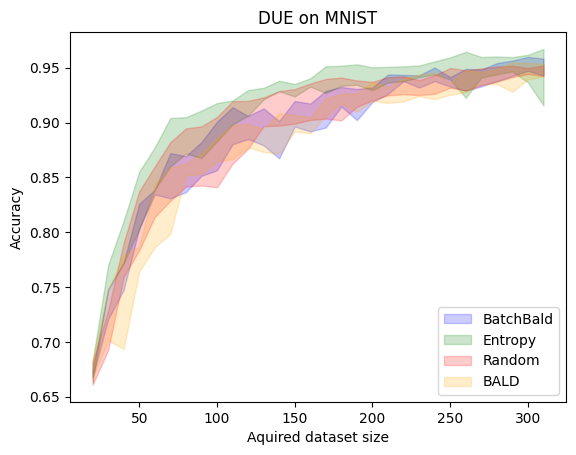
\includegraphics[scale=0.75]{random.png}
\caption{Random MNIST}
\end{figure}

\subsubsection{Unbalanced MNIST (DNN vs BNN vs DUE)}

\begin{figure}[H]
\centering
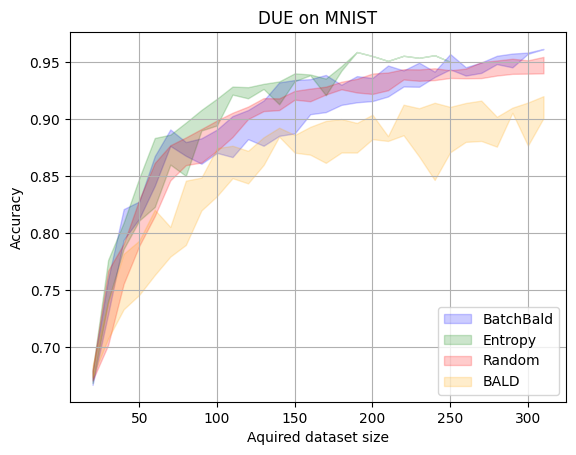
\includegraphics[scale=1]{Unbalanced.png}
\caption{Random Unbalanced MNIST}
\end{figure}
\subsubsection{Repeated MNIST (DNN vs BNN vs DUE)}

\begin{figure}[H]
\centering
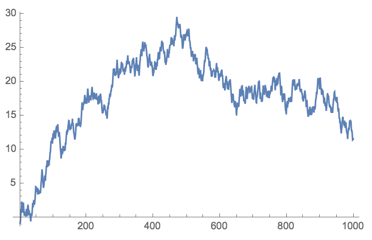
\includegraphics[scale=1]{todo.png}
\caption{Random Repeated MNIST}
\end{figure}

\subsection{BALD}

\subsubsection{MNIST (BNN vs DUE)}

\begin{figure}[H]
\centering
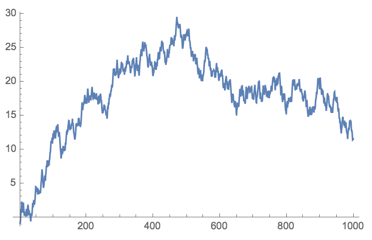
\includegraphics[scale=1]{todo.png}
\caption{BALD MNIST}
\end{figure}

\subsubsection{Unbalanced MNIST (BNN vs DUE)}

\begin{figure}[H]
\centering
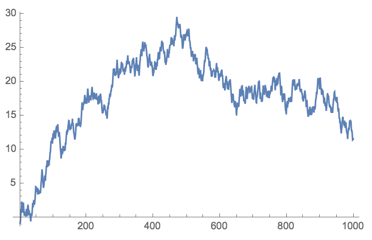
\includegraphics[scale=1]{todo.png}
\caption{BALD Unbalanced MNIST}
\end{figure}

\subsubsection{Repeated MNIST (BNN vs DUE)}

\begin{figure}[H]
\centering
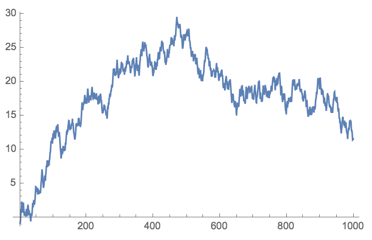
\includegraphics[scale=1]{todo.png}
\caption{BALD Repeated MNIST}
\end{figure}
    

\subsection{BatchBALD}

\subsubsection{MNIST (BNN vs DUE)}

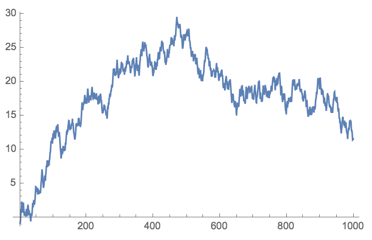
\includegraphics{todo.png}

\subsubsection{Unbalanced MNIST (BNN vs DUE)}

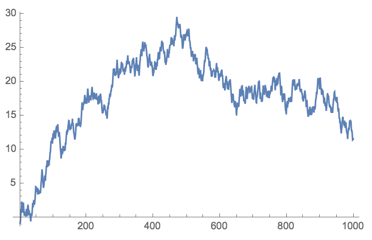
\includegraphics{todo.png}

\subsubsection{Repeated MNIST (BNN vs DUE)}

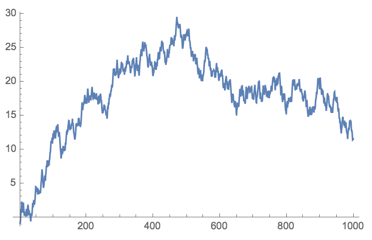
\includegraphics{todo.png}


\subsection{Joint Entropy}

\subsubsection{MNIST (BNN vs DUE)}

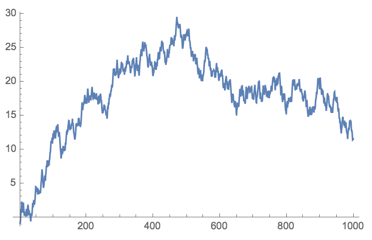
\includegraphics{todo.png}

\subsubsection{Unbalanced MNIST (BNN vs DUE)}

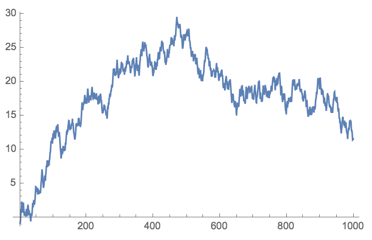
\includegraphics{todo.png}

\subsubsection{Repeated MNIST (BNN vs DUE)}

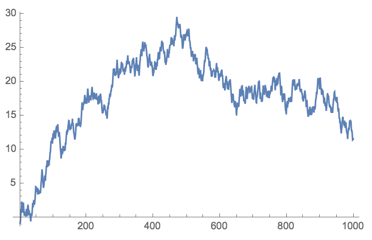
\includegraphics{todo.png}




\section{Interpretation of results}

The outline of the results from these experiments as as follows.

\begin{itemize}
    \item The specific failure modes of BALD and Random which we tested for occur when using DUE, much like when using a BNN
    \item The performance of simply using the joint entropy of the output variables leads to superior performance than the use of the BatchBALD objective when working with DUE. This is not observed when using BNNs.
\end{itemize}


\subsection{Qualitative results at the acquired batches}

See \hyperref[sec:Batches]{appendices} for a wider selection of acquired batches for the various active learning method.

We can view the batches and the sorts of datapoints which they select. As we would expect from the BALD acquisition function we get points which are quite similar all selected in the same batch.

\begin{figure}[H]
    \centering
    \includegraphics[scale=0.75]{bald/3.png}
    \caption{BALD selected batch}
\end{figure}


The randomly selected datapoints are not very useful to observe but are included in the appendices for completeness.

\begin{figure}[H]
    \centering
    \begin{subfigure}[b]{0.3\textwidth}
        \centering
        \includegraphics[width=\textwidth]{entropy/3.png}
        \caption{Entropy selected batch}
    \end{subfigure}
    \hfill
    \begin{subfigure}[b]{0.3\textwidth}
        \centering
        \includegraphics[width=\textwidth]{batchbald/3.png}
        \caption{BatchBALD selected batch}
    \end{subfigure}
\end{figure}

We can qualitatively observe that the points which the entropy method selects are diverse, as are the points selected by BatchBALD. BatchBALD selects points which are similar but the model believes could be of distinct classes. The 3 and 8 selected look similar but are of 2 different classes.


\subsection{Entropy vs BatchBALD for DUE}


From our experiments we can observe that using the joint entropy alone performs better than the BatchBALD objective. Here we will explore one reason why this maybe the case.

The difference between the 2 objectives is that with the BatchBALD objective we are subtracting the conditional entropy from the 

The motivation for the BALD objective in the original paper where it was introduced \cite{houlsby2011bayesian}, is to select the point which maximally reduce the uncertainty over the hypothesis space.

\subsubsection{Conditional Entropy}

The second part of the BALD object is the conditional entropy of the output variable conditioned on the function value. The output length scale of our model is a learned parameter of our model. When our GPs on the feature space reverts to the prior, the conditional entropy will become a function of the output scale of the GP.

All of the covariance matrices will be scaled by this output length scale, and the value of the conditional entropy is very dependent on this value.

We can demonstrate the possible issue with this, with the following example where we have a uniform belief about the output of the random variable but we change the length scale of our model.



\section{Future Extensions}

In this project report we have created a working framework for Batch active learning with Deep Kernel Gaussian Processes Classifiers. We have reduced the computational complexity of these methods so they are computational feasible. We have also verified that this approach is SOTA.





\renewcommand{\bibname}{Bibliography}
\bibliographystyle{apacite}
\bibliography{Bibliography.bib}

\begin{appendices}
\chapter{Appendix}

\section{Examples of selected batches}
\label{sec:Batches}

These are examples of the first 6 batches acquired by the various active learning methods on a particular run.

\subsection{DUE}

\subsubsection{Entropy}
\includegraphics{entropy/1.png}
\includegraphics{entropy/2.png}
\includegraphics{entropy/3.png}
\includegraphics{entropy/4.png}
\includegraphics{entropy/5.png}
\includegraphics{entropy/6.png}


\subsubsection{BALD}
\includegraphics{bald/1.png}
\includegraphics{bald/2.png}
\includegraphics{bald/3.png}
\includegraphics{bald/4.png}
\includegraphics{bald/5.png}
\includegraphics{bald/6.png}

\subsubsection{BatchBALD}
\includegraphics{batchbald/1.png}
\includegraphics{batchbald/2.png}
\includegraphics{batchbald/3.png}
\includegraphics{batchbald/4.png}
\includegraphics{batchbald/5.png}
\includegraphics{batchbald/6.png}

\section{Training Curves}

\section{Derivation of Natural Gradient Descent}

\end{appendices}

\end{document}